
\subsection{Test Plan Objectives}
This document describes the testing done on the patient handling software produced by HeartByte for our customer Region Östergötland. This document should map the test making procedure aswell as the Software Testing Life Cycle where the initiation of tests, the definition of tests and the design of the tests are described. This testplan will follow the structure provided by guru99 [1].

\subsection{Scope}
\subsubsection{In Scope}

\begin{itemize}
  \item Functional Requirements
\end{itemize}
  \vfill
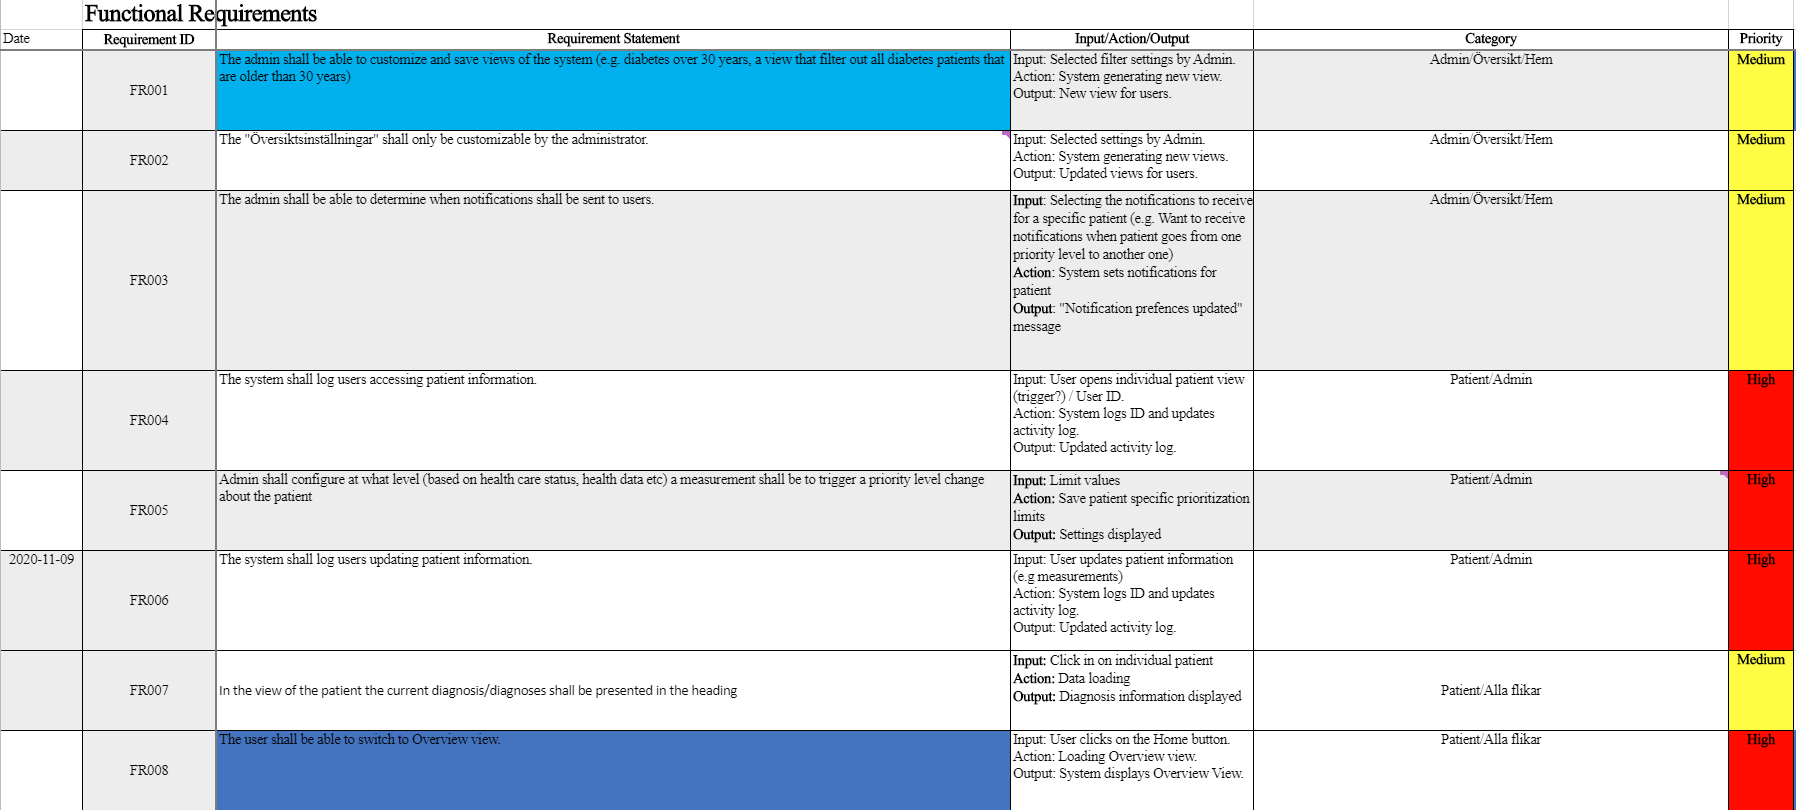
\includegraphics[width=\linewidth]{Pictures/Func1} (1)

    \vfill
    \vfill
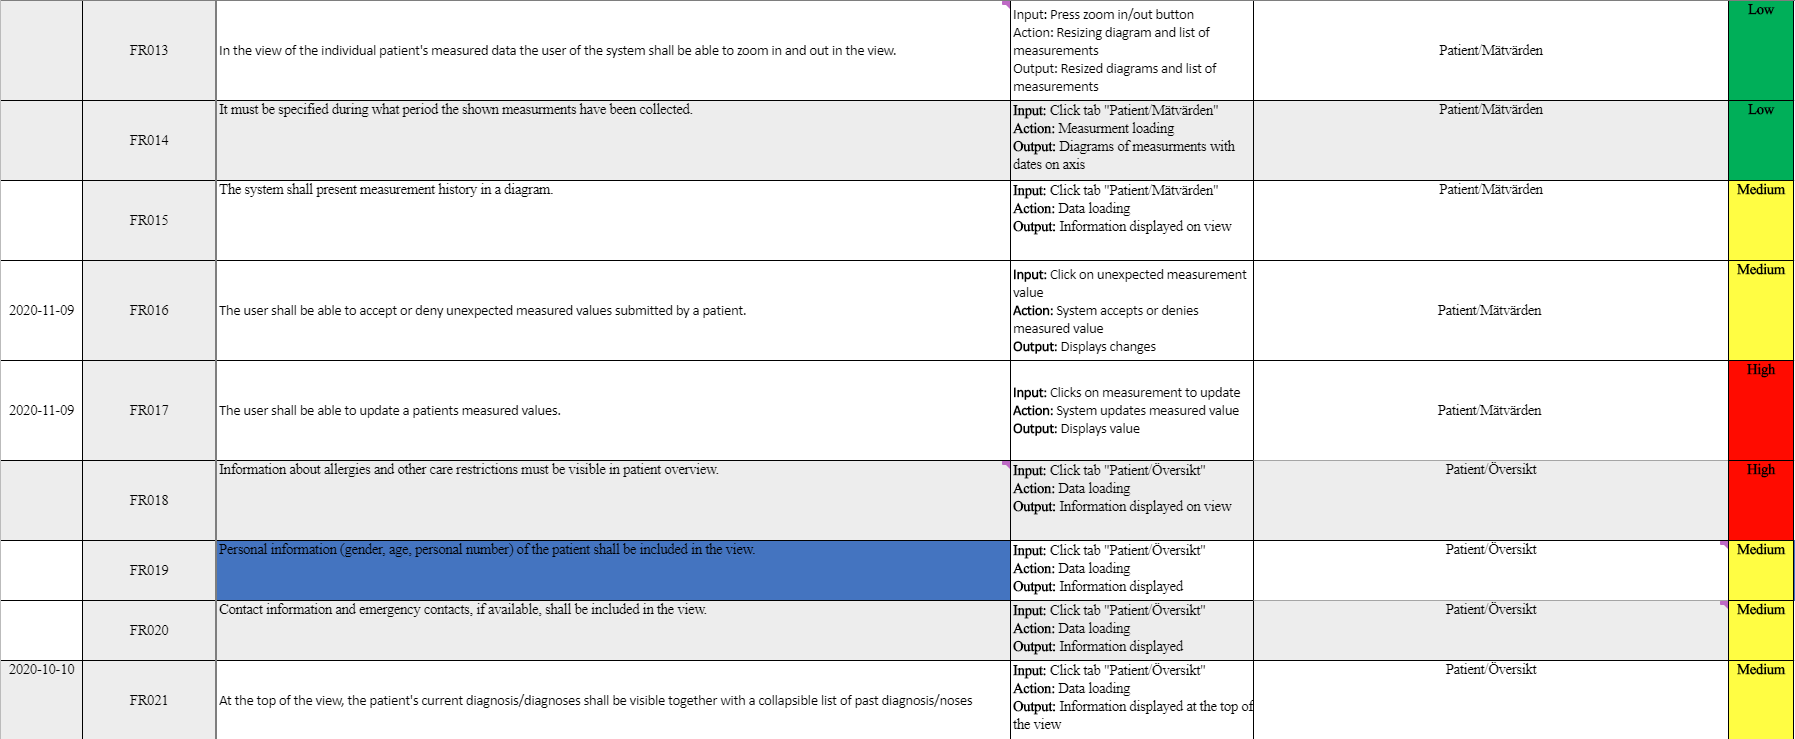
\includegraphics[width=\linewidth]{Pictures/Func2} (2)

    \vfill
\clearpage
\begin{itemize}
    \item Non-Functional Requirements 
\end{itemize}
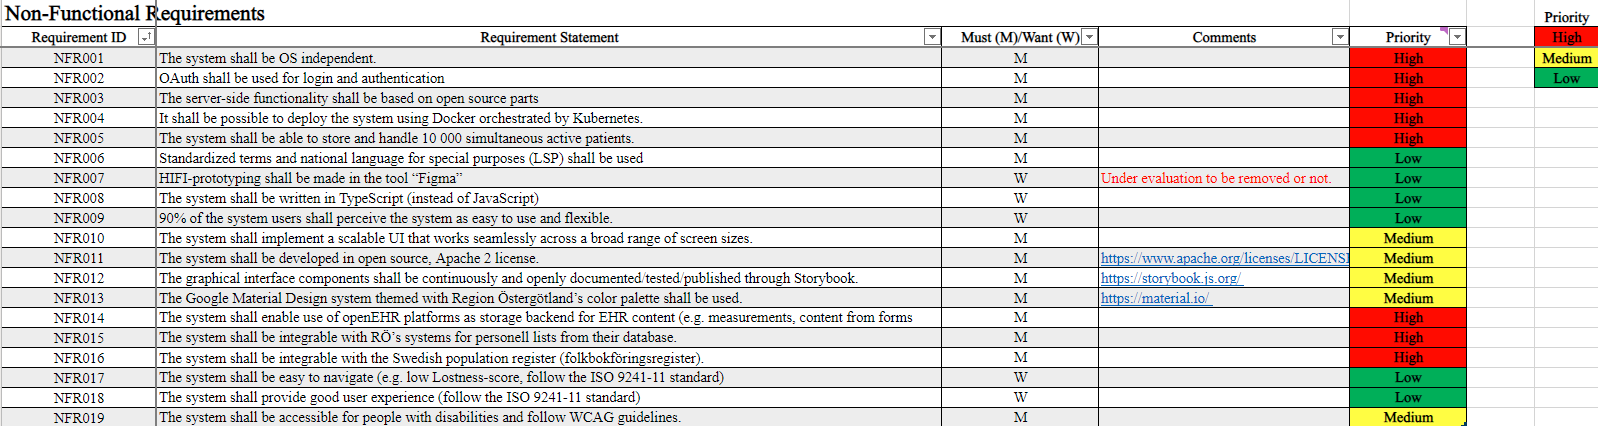
\includegraphics[width=\linewidth]{Pictures/Nonfunc.PNG} (3)

    \vfill
*Both the Functional and non-functional requirements can be found as larger pictures in Appendix A.
  
  


\subsubsection{Out of Scope (needs more specification)}
Anything outside of our requirements and functionality will not be tested. OpenEHR will only have output tests since we can't manage the DB ourselves.
\subsection{Quality Objective}
To ensure that our application will meet the requirements and user tests provided by Region Östergötland. This means both the Functional and non functional requirements. 

To ensure that Bugs and issues are identified using a bug tracking system (TBD) and is continuously checked for bugs.

Using a CI in the Gitlab client to ensure that our code meets the functionality standard set by our automatic tests. By ensuring our CI Heartbyte is looking to implement Continuous Delivery by doing small updates to the software, instead of large feature updates. 
\subsection{Roles}
\begin{flushleft}
   \textbf{Test Leader}
    
    
    Gustav Karlsson
  
   \textbf{Tester}
   
    Hjalmar Svensson
    
    Mattis Bark
   
   
   \textbf{Quality Coordinator}
   
    Emma Johansson
     

\end{flushleft}

\subsection{References}
\begin{enumerate}
  \item https://www.guru99.com/test-plan-for-project.html
  \item https://www.ida.liu.se/~TDDC88/theory/07esting.pdf
\end{enumerate}
